\chapter{Revisi\'on de Sistemas Operativos}
\section{GNU/Linux}

\subsection{Historia y Propósito}
\textcite{gnu-project} anunciaron en 1983 el \textit{Proyecto GNU}, cuyo propósito era desarrollar 
un sistema operativo libre y compatible con Unix. Sin embargo, no contaba con un núcleo funcional 
hasta que Linus Torvalds liberó en 1991 el \textit{kernel} Linux, que en 1992 adoptó la licencia GPL.  
La combinación de GNU y Linux dio origen a \textbf{GNU/Linux}, usado ampliamente en servidores, 
supercomputadoras y sistemas de escritorio \parencite{debian-history}.  

\subsection{Arquitectura}
El kernel de Linux adopta una arquitectura \textbf{monolítica}, 
donde procesos, memoria, E/S, sistemas de archivos y comunicación entre procesos se ejecutan en un único espacio privilegiado.  
No obstante, mantiene modularidad mediante \textit{módulos del kernel} que pueden cargarse dinámicamente 
en tiempo de ejecución \parencite{kernel-docs}.  

\begin{figure}[H]
  \centering
  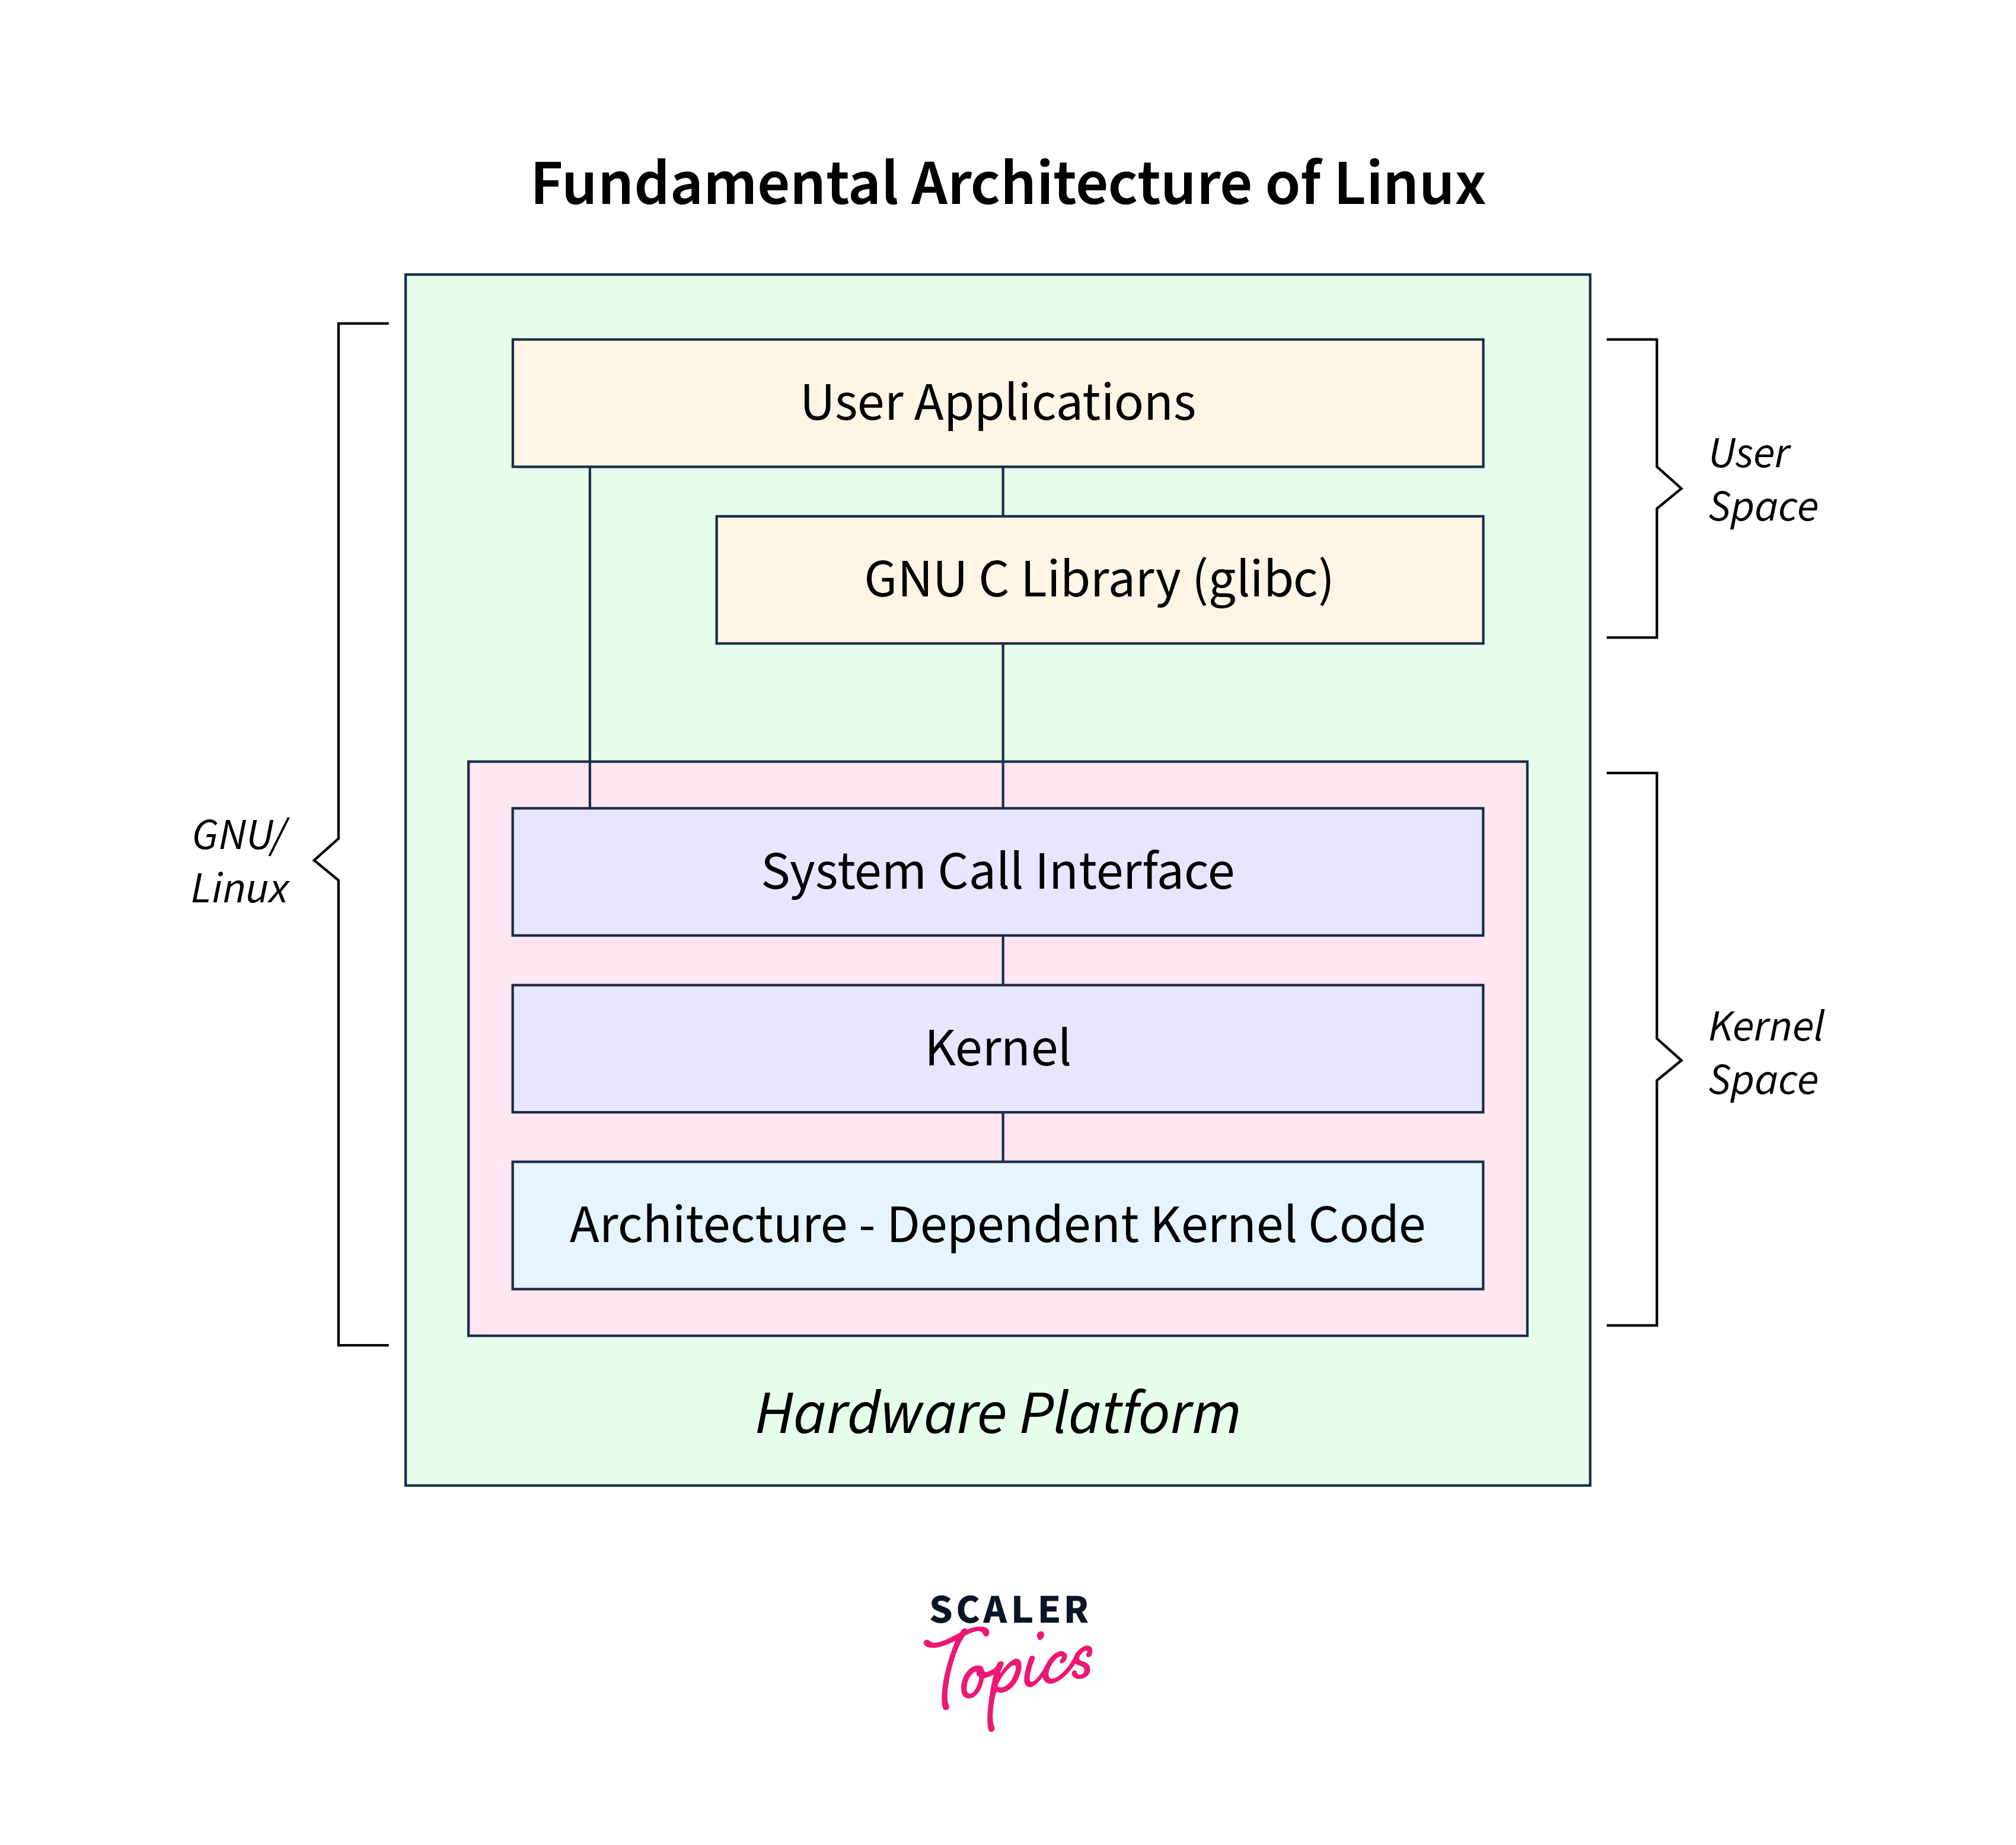
\includegraphics[width=0.75\textwidth]{figures/gnu-linux-arq.png}
  \caption[GNU/Linux: arquitectura]{Arquitectura del kernel de GNU/Linux (monolítico ). Extraído de \parencite{kernel-docs}.}
  \label{fig:arq-gnu-linux}
\end{figure}

\subsection{Lenguaje de Implementación}
El núcleo está escrito principalmente en \textbf{C} (dialecto GNU de C11) para garantizar eficiencia y portabilidad.  
En secciones críticas emplea ensamblador, y desde la versión 6.1 incluye soporte experimental para \textbf{Rust}, 
destinado a \textit{drivers} y módulos más seguros \parencite{kernel-docs}.  


\subsection{Componentes Clave}

\begin{table}[H]
\centering
\begin{tabular}{p{3.2cm}p{5cm}p{6cm}}
\hline
\textbf{Componente} & \textbf{Función principal} & \textbf{Detalles clave / ejemplos} \\
\hline
Gestión de procesos & Coordinar la creación, destrucción y planificación de procesos & Soporta multitarea preventiva; usa el \textit{Completely Fair Scheduler}; incluye sincronización, señales e hilos de kernel \\
\hline
Gestión de memoria & Administrar el acceso a la memoria principal y secundaria & Implementa \textit{memoria virtual}, paginación, swapping y memoria compartida; optimiza con \textit{caching} \\
\hline
Sistemas de archivos & Abstraer diferentes formatos de almacenamiento bajo una interfaz unificada & Proporciona el \textit{Virtual File System} (VFS); soporta EXT4, FAT, NTFS, XFS, NFS, entre otros \\
\hline
Drivers & Facilitar la comunicación entre el kernel y el hardware & Incluye controladores para dispositivos de red, almacenamiento, gráficos y sonido; los módulos son cargables dinámicamente \\
\hline
Red e IPC & Manejar la comunicación entre procesos y la conectividad en red & Implementa pila TCP/IP, sockets, colas de mensajes, semáforos y memoria compartida para IPC \\
\hline
\end{tabular}
\caption[Componentes y funciones clave del kernel de GNU/Linux]{Componentes y funciones principales del kernel de GNU/Linux. Basado en \textcite{tldp,kernel-docs}.}
\label{tab:componentes-gnu-linux}
\end{table}


\subsection{Comunidad y Documentación Disponible}
El desarrollo de GNU/Linux está coordinado por Linus Torvalds y mantenedores del kernel, 
junto a miles de colaboradores en universidades y empresas.  
La documentación oficial está disponible en \textit{kernel.org}, complementada por proyectos como el 
\textit{Linux Documentation Project} y las guías de distribuciones como Debian o Ubuntu \parencite{linux-foundation}.



\section{FreeBSD}

\subsection{Historia y Propósito}
\textcite{freebsd-history} explican que FreeBSD nació en 1993 como continuación del sistema BSD de la Universidad de California en Berkeley.  
Su propósito ha sido ofrecer un sistema operativo libre, robusto y con licencia permisiva (BSD), lo que permitió su adopción en investigación, servidores y productos comerciales.  
A diferencia de GNU/Linux, FreeBSD mantiene una integración completa entre kernel y userland, publicándose como un sistema operativo completo \parencite{freebsdfoundation}.  

\begin{figure}[H]
  \centering
  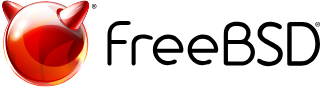
\includegraphics[width=0.75\textwidth]{figures/freebsd-logo.png}
  \caption[FreeBSD: logotipo]{Logotipo oficial de FreeBSD. Extraído de \parencite{freebsdfoundation}.}
  \label{fig:logo-freebsd}
\end{figure}


\subsection{Arquitectura}
El kernel de FreeBSD es \textbf{monolítico con modularidad}, integrando gestión de procesos, memoria, redes y sistemas de archivos en un único espacio de kernel, pero permitiendo cargar módulos en tiempo de ejecución.  
Incluye una pila de red avanzada, soporte para arquitecturas múltiples y compatibilidad binaria con ejecutables de Linux \parencite{freebsd-arch}.

\begin{figure}[htbp]
  \centering
  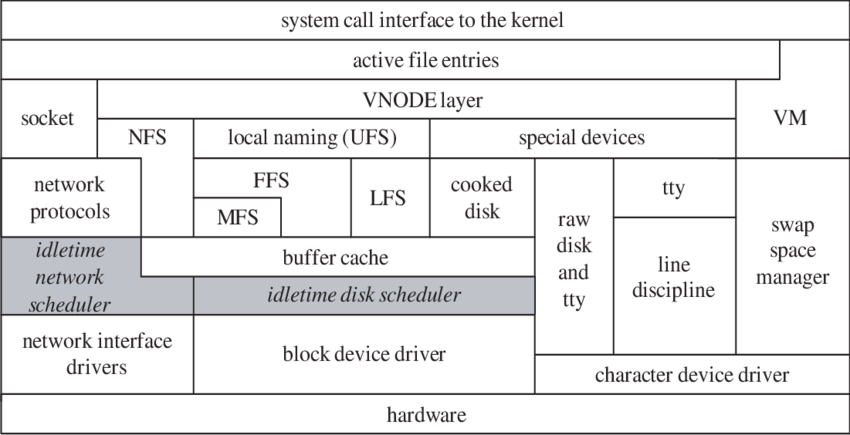
\includegraphics[width=0.75\textwidth]{figures/freebsd_kernel_io.png}
  \caption[Esquema de la gestión de E/S en el kernel de FreeBSD]{Esquema de la gestión de E/S en el kernel de FreeBSD, adaptado de McKusick (1996) \parencite{freebsd_kernel_io}.}
  \label{fig:freebsd_kernel_io}
\end{figure}


\subsection{Lenguaje de Implementación}
El núcleo está escrito principalmente en \textbf{C}, con secciones en ensamblador para funciones críticas y utilidades en userland.  
La documentación oficial resalta la portabilidad y mantenibilidad del código, lo que ha facilitado su adaptación a procesadores x86, ARM, PowerPC y más \parencite{freebsd-docs}.  

\subsection{Componentes Clave}



\begin{table}[H]
\centering
\begin{tabular}{p{3.2cm}p{5cm}p{6cm}}
\hline
\textbf{Componente} & \textbf{Función principal} & \textbf{Detalles clave / ejemplos} \\
\hline
Gestión de procesos y memoria & Coordinar la ejecución de procesos y la administración de memoria & Soporta multitarea, planificación avanzada y memoria virtual; permite alta estabilidad en servidores \\
\hline
Sistemas de archivos & Proveer soporte de almacenamiento con múltiples formatos & Incluye UFS (nativo), ZFS (robusto y escalable), además de otros mediante VFS \\
\hline
Redes & Manejar conectividad y seguridad en red & Dispone de una pila TCP/IP avanzada, soporte para IPv6 y mecanismos como firewalls (pf, ipfw) \\
\hline
Módulos y drivers & Extender la compatibilidad con hardware moderno & Los controladores pueden cargarse dinámicamente; amplio soporte para arquitecturas como x86, ARM y PowerPC \\
\hline
Userland & Ofrecer utilidades y herramientas integradas al sistema & Incluye las herramientas BSD clásicas; FreeBSD se publica como un sistema completo (kernel + userland) \\
\hline
\end{tabular}
\caption[Componentes y funciones clave del kernel de FreeBSD]{Componentes y funciones principales del kernel y sistema FreeBSD. Basado en \textcite{freebsd-docs,freebsdfoundation}.}
\label{tab:componentes-freebsd}
\end{table}


\subsection{Comunidad y Documentación Disponible}
El desarrollo de FreeBSD está gestionado por el \textit{Core Team} y la \textit{FreeBSD Foundation}, con aportes de universidades, empresas y voluntarios.  
La documentación se centraliza en el \textit{FreeBSD Handbook}, manuales técnicos y páginas de manual (\textit{man pages}), siendo una de las guías más completas en sistemas Unix \parencite{freebsdfoundation}.


\section{Minix 3}

\subsection{Historia y Propósito}
\textcite{tanenbaum-history} señalan que Minix fue creado en 1987 por Andrew S. Tanenbaum como un sistema educativo para la enseñanza de sistemas operativos.  
En 2005 se presentó \textbf{Minix 3}, una versión orientada a la confiabilidad y al uso en sistemas embebidos, con un diseño ligero y tolerante a fallos.  
Su propósito central es ofrecer un sistema operativo de código abierto, sencillo y seguro, que pueda reiniciar controladores defectuosos sin afectar al núcleo \parencite{minix3site}.  

\subsection{Arquitectura}
El núcleo de Minix 3 sigue el modelo de \textbf{microkernel}, en el cual las funciones esenciales como planificación, comunicación entre procesos (IPC) y gestión básica de memoria se ejecutan en el kernel, mientras que servicios como el sistema de archivos, controladores y gestión de red se ejecutan en espacio de usuario \parencite{minix3-design}.  
Este diseño busca maximizar la estabilidad, ya que los fallos en drivers no comprometen el sistema completo.  

\begin{figure}[H]
  \centering
  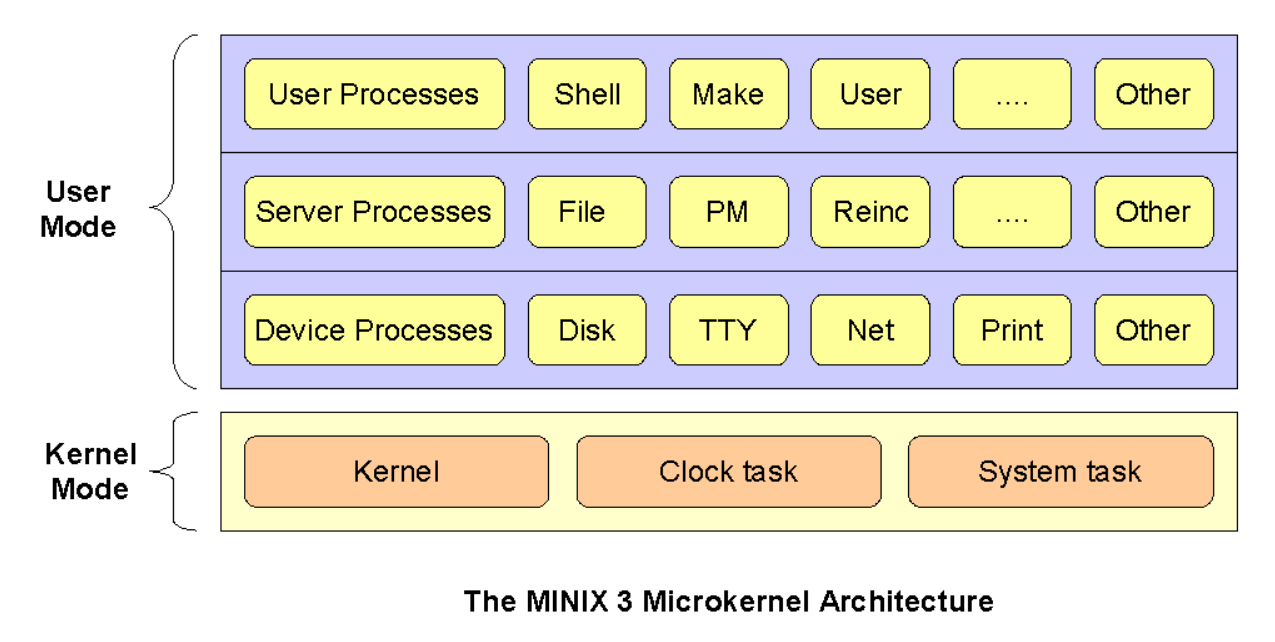
\includegraphics[width=1.05\textwidth]{figures/minix3-arq.png}
  \caption[Minix 3: arquitectura]{Arquitectura de Minix 3 (microkernel + servidores en espacio de usuario). Extraído de \parencite{minix3-design}.}
  \label{fig:arq-minix3}
\end{figure}

\subsection{Lenguaje de Implementación}
Minix 3 está escrito principalmente en \textbf{C}, con pequeñas partes en ensamblador.  
La implementación prioriza la claridad y simplicidad del código, lo que lo hace ideal como plataforma de investigación y docencia \parencite{minix3-docs}.  

\subsection{Componentes Clave}
De acuerdo con \textcite{minix3-docs}, los principales componentes de Minix 3 son:

\begin{table}[H]
\centering
\begin{tabular}{p{3.2cm}p{5cm}p{6cm}}
\hline
\textbf{Componente} & \textbf{Función principal} & \textbf{Detalles clave / ejemplos} \\
\hline
Microkernel & Coordinar lo esencial del sistema & Gestiona planificación de procesos, comunicación entre procesos (IPC) y manejo de interrupciones \\
\hline
Servers en espacio de usuario & Ejecutar servicios del sistema fuera del núcleo & Incluyen sistemas de archivos, controladores de dispositivos y gestión de red, todos en espacio de usuario para mayor seguridad \\
\hline
Gestión de fallos & Asegurar la confiabilidad del sistema & Permite el reinicio automático de drivers defectuosos sin necesidad de reiniciar todo el sistema \\
\hline
Herramientas y librerías & Proveer un entorno de desarrollo completo y estandarizado & Incluye utilidades POSIX, compiladores y librerías que facilitan la portabilidad de aplicaciones \\
\hline
\end{tabular}
\caption[Componentes y funciones clave de Minix 3]{Componentes y funciones principales de Minix 3. Basado en \textcite{minix3-docs}.}
\label{tab:componentes-minix3}
\end{table}


\subsection{Comunidad y Documentación Disponible}
El desarrollo de Minix 3 está coordinado por la Vrije Universiteit Amsterdam con apoyo de colaboradores internacionales.  
El proyecto mantiene como referencia principal el sitio oficial \textit{minix3.org}, la documentación técnica, el \textit{Design Document} y los manuales para usuarios y desarrolladores \parencite{minix3site}.  
 

\section{Redox OS}

\subsection{Historia y Propósito}
\textcite{redox-os} explican que Redox OS es un sistema operativo iniciado en 2015 con el objetivo 
de ofrecer una alternativa moderna y segura basada en un \textbf{microkernel} escrito en Rust.  
Su propósito es combinar la filosofía de sistemas Unix con la seguridad en memoria de Rust, 
evitando fallos comunes en C y C++. Además, busca servir como plataforma educativa y práctica 
para investigación en sistemas operativos \parencite{redox-docs}. 

\begin{figure}[H]
  \centering
  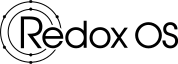
\includegraphics[width=0.5\textwidth]{figures/redox-logo.png}
  \caption[Redox OS: logotipo]{Logotipo oficial de Redox OS. Extraído de \parencite{redox-os}.}
  \label{fig:logo-redox}
\end{figure}


\subsection{Arquitectura}
El núcleo de Redox OS adopta un diseño \textbf{microkernel}, en el cual los controladores, 
sistemas de archivos y servicios de red se ejecutan en espacio de usuario, reduciendo 
los riesgos de fallos críticos. La interfaz principal de comunicación es el sistema de 
mensajes y canales, inspirado en microkernels como Minix y seL4 \parencite{redox-book}. 

\begin{figure}[H]
  \centering
  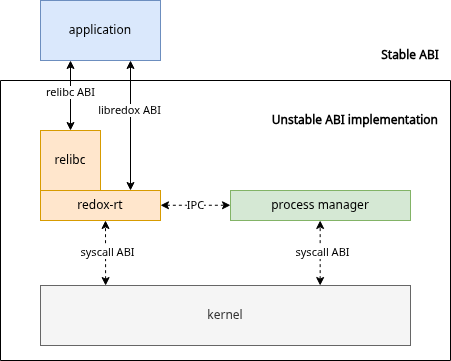
\includegraphics[width=0.75\textwidth]{figures/redox_kernel_abi.png}
  \caption[Esquema de la ABI en Redox OS]{Esquema de la ABI en Redox OS y el manejo de llamadas al sistema en espacio de usuario \parencite{redox_kernel11}.}
  \label{fig:redox_kernel_abi}
\end{figure}

\subsection{Lenguaje de Implementación}
Todo el sistema está implementado en \textbf{Rust}, lenguaje que previene errores de memoria 
y garantiza concurrencia segura. Esto representa un cambio respecto a los kernels clásicos 
en C, ofreciendo mayor robustez y confiabilidad \parencite{redox-github}.  

\subsection{Componentes Clave}
De acuerdo con \textcite{redox-docs}, los principales componentes de Redox OS son:

\begin{table}[H]
\centering
\begin{tabular}{p{3.2cm}p{5cm}p{6cm}}
\hline
\textbf{Componente} & \textbf{Función principal} & \textbf{Detalles clave / ejemplos} \\
\hline
Microkernel & Proveer los servicios esenciales del sistema & Incluye planificación, gestión básica de memoria y comunicación entre procesos (IPC) \\
\hline
Sistemas de archivos & Unificar el acceso a recursos bajo un mismo esquema & Inspirado en Plan 9; jerarquía unificada para archivos, dispositivos y procesos \\
\hline
Drivers & Gestionar el hardware de forma segura y modular & Implementados en espacio de usuario; mayor aislamiento y tolerancia a fallos frente a errores en controladores \\
\hline
Librería estándar & Ofrecer una base para el desarrollo de aplicaciones y programas del sistema & \texttt{relibc}, escrita en Rust, alternativa moderna y segura a \texttt{glibc} \\
\hline
\end{tabular}
\caption[Componentes y funciones clave de Redox OS]{Componentes y funciones principales de Redox OS. Basado en \textcite{redox-docs}.}
\label{tab:componentes-redox}
\end{table}


\subsection{Comunidad y Documentación Disponible}
El desarrollo de Redox OS está coordinado en GitHub por Jeremy Soller y una comunidad activa de colaboradores.  
La documentación se organiza en el \textit{Redox Book}, artículos técnicos y guías prácticas, 
junto al repositorio oficial donde se gestionan los avances y propuestas \parencite{redox-github}.


\section{Microsoft Windows}

\subsection{Historia y Propósito}
\textcite{windows-history} señalan que Windows nació en 1985 como una extensión gráfica de MS-DOS, 
y evolucionó hasta convertirse en un sistema operativo independiente a partir de Windows NT (1993).  
Su propósito ha sido proveer una plataforma comercial con interfaz gráfica, compatibilidad con software 
existente y soporte para aplicaciones empresariales y de usuario final \parencite{microsoftdocs}.  

\subsection{Arquitectura}
El núcleo moderno de Windows (NT Kernel) es \textbf{híbrido}, combinando características de microkernel 
y monolítico. Incluye el \textit{Executive} (gestión de memoria, procesos y seguridad), el \textit{Kernel} 
(planificación de hilos e interrupciones) y subsistemas en espacio de usuario que proveen compatibilidad POSIX 
y Win32 \parencite{russinovich}.  

\begin{figure}[H]
  \centering
  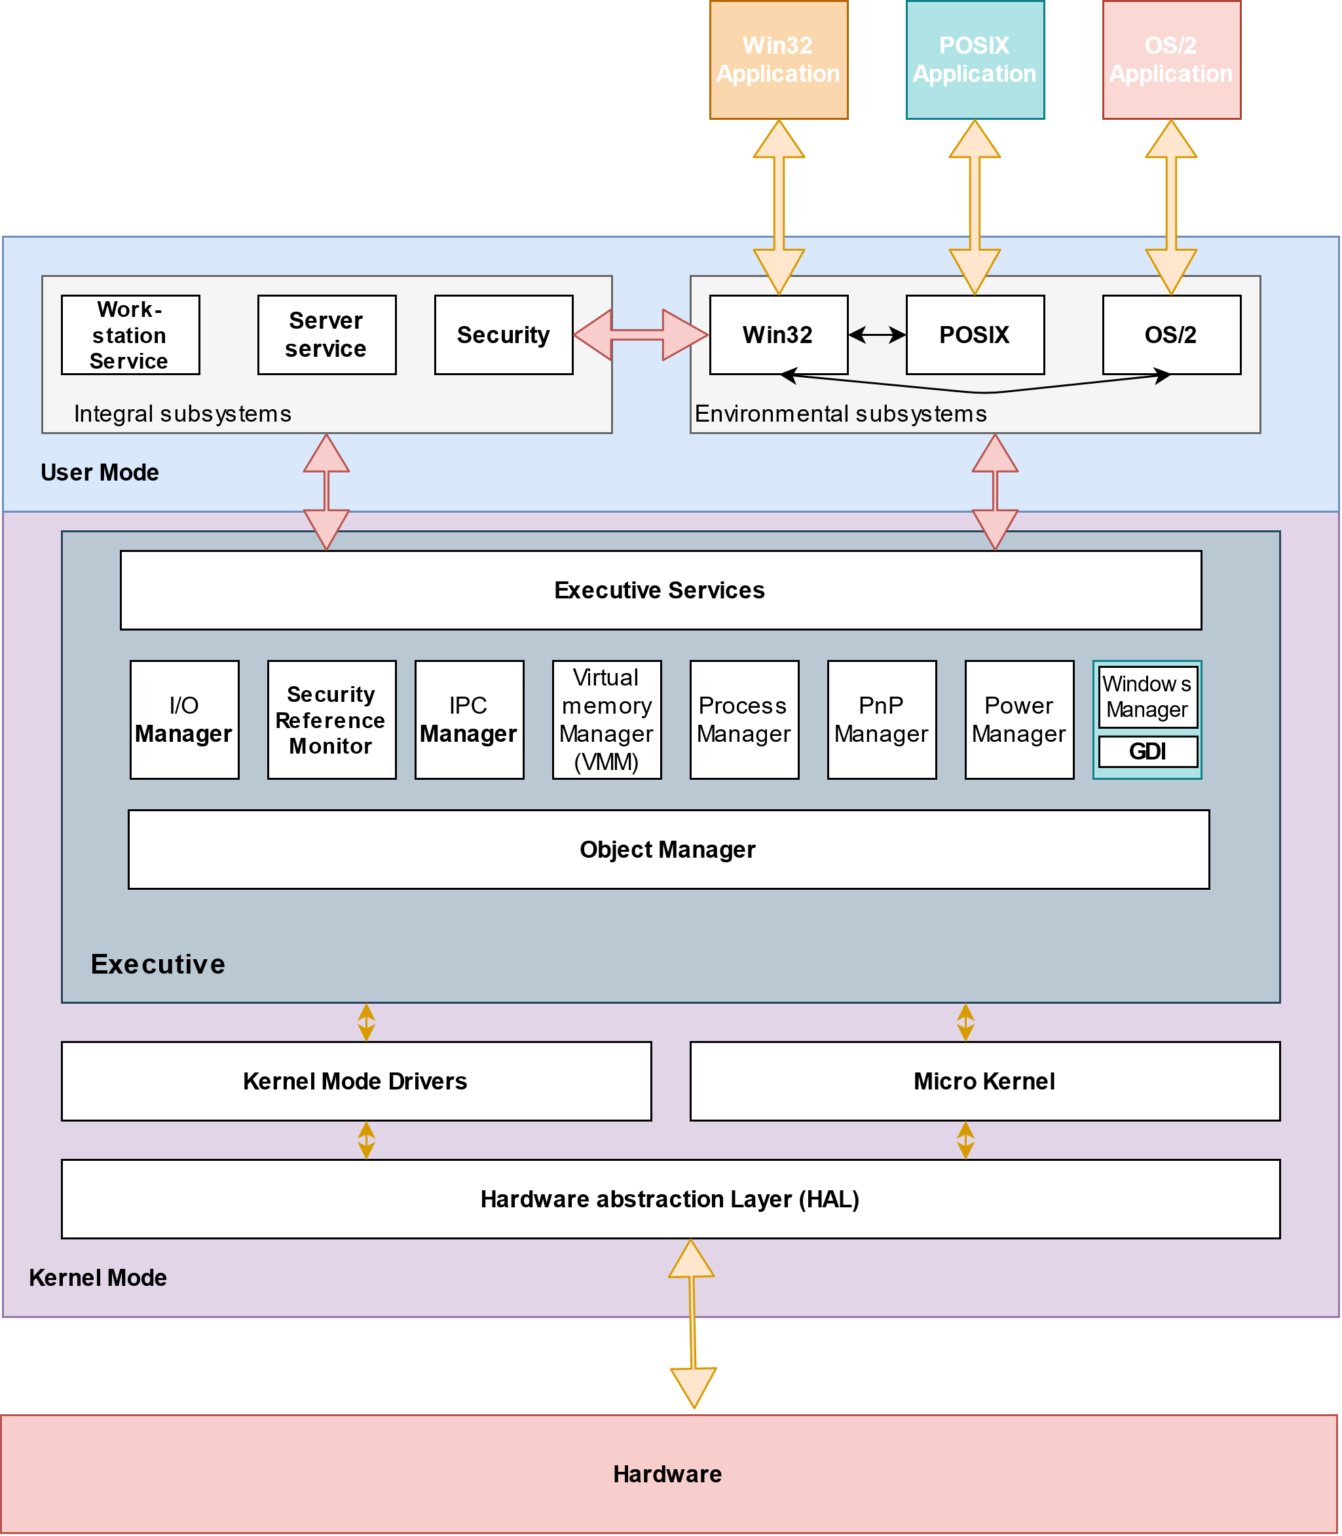
\includegraphics[width=0.75\textwidth]{figures/windows-nt-arch.png}
  \caption[Windows NT: arquitectura]{Arquitectura del sistema operativo Windows NT (núcleo híbrido). Extraído de \parencite{russinovich}.}
  \label{fig:arq-windows}
\end{figure}


\subsection{Lenguaje de Implementación}
El sistema está implementado principalmente en \textbf{C y C++}, con secciones críticas en ensamblador.  
Componentes de alto nivel como la interfaz gráfica y bibliotecas modernas utilizan C++ y C\#.  
La documentación de Microsoft destaca su diseño modular y adaptable a diversas arquitecturas \parencite{microsoftdocs}.  

\subsection{Componentes Clave}

\begin{table}[H]
\centering
\begin{tabular}{p{3.2cm}p{5cm}p{6cm}}
\hline
\textbf{Componente} & \textbf{Función principal} & \textbf{Detalles clave / ejemplos} \\
\hline
Kernel y Executive & Gestionar procesos, memoria y seguridad del sistema & Incluye planificación de hilos, sincronización, control de accesos y mecanismos de seguridad en el núcleo \\
\hline
Subsistemas & Garantizar compatibilidad con distintas aplicaciones & Win32 (principal), compatibilidad con POSIX y emulación de DOS; permite ejecutar software heredado \\
\hline
Sistemas de archivos & Administrar almacenamiento con distintos formatos & Soporta NTFS (avanzado y seguro), FAT y exFAT (usados en dispositivos externos) \\
\hline
Drivers & Conectar el sistema operativo con el hardware & Modelo WDM (Windows Driver Model); soporte para dispositivos modernos con carga dinámica de controladores \\
\hline
Interfaz gráfica & Proporcionar entorno visual e interacción con el usuario & Basada en GDI (\textit{Graphics Device Interface}) y DirectX para gráficos avanzados y multimedia \\
\hline
\end{tabular}
\caption[Componentes y funciones clave de Windows]{Componentes y funciones principales del sistema operativo Windows. Basado en \textcite{russinovich}.}
\label{tab:componentes-windows}
\end{table}


\subsection{Comunidad y Documentación Disponible}
El desarrollo de Windows es gestionado por Microsoft, con participación de socios comerciales y fabricantes 
de hardware. La documentación oficial está disponible en el portal \textit{Microsoft Learn} (Microsoft Docs), 
junto con libros como \textit{Windows Internals}, que sirven de referencia académica y técnica \parencite{microsoftdocs}.
 

%-----------------------------------------------------------------------------------
%-----------------------------------------------------------------------------------
\section{SerenityOS}

\subsection{Historia y Propósito}
SerenityOS fue iniciado en 2018 por Andreas Kling como un proyecto personal 
enfocado en recrear un sistema operativo desde cero, inspirado en la estética 
y simplicidad de los entornos de los años 90 \parencite{serenityos:website}.
El objetivo es combinar productividad con entretenimiento, sirviendo además 
como plataforma de experimentación en investigación y enseñanza por su código claro 
y diseño accesible. \textcite{serenityos_adafruit} explican que el sistema recrea la experiencia 
nostálgica de los sistemas operativos clásicos con tecnología moderna.

\begin{figure}[H]
  \centering
  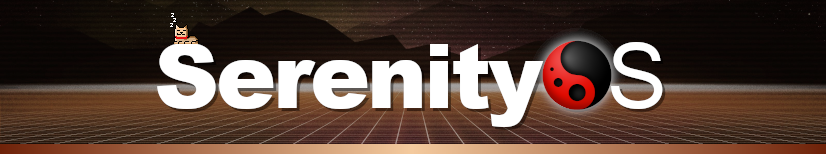
\includegraphics[width=0.75\textwidth]{figures/serenityos-logo.png}
  \caption[SerenityOS: logotipo]{Logotipo oficial de SerenityOS. Extraído de \parencite{serenityos:website}.}
  \label{fig:logo-serenityos}
\end{figure}


\subsection{Arquitectura}
El núcleo de SerenityOS es un kernel monolítico estilo Unix de 64 bits, 
que gestiona procesos, memoria virtual, dispositivos y temporizadores 
de manera centralizada \parencite{serenityos:github}. 
Sobre él se construye un sistema de ventanas propio y librerías POSIX internas, 
lo que refuerza la idea de una arquitectura monolítica con servicios integrados.

\subsection{Lenguaje de Implementación}
El sistema está implementado en C++20 moderno, evitando el uso de STL 
en favor de una biblioteca estándar propia, lo que le permite 
un control detallado de la memoria y el comportamiento del kernel y 
de sus aplicaciones, como detallan los desarrolladores del proyecto \parencite{serenityos:github}.

\subsection{Componentes Clave}
De acuerdo a la documentación técnica y al repositorio oficial, los principales componentes son:
\begin{table}[H]
\centering
\begin{tabular}{p{3.2cm}p{5cm}p{6cm}}
\hline
\textbf{Componente} & \textbf{Función principal} & \textbf{Detalles clave / ejemplos} \\
\hline
Gestión de memoria & Administrar memoria física y virtual del sistema & Soporte de memoria virtual con su propio asignador eficiente; inspirado en diseños tipo Unix \\
\hline
Sistema de archivos & Manejar almacenamiento con compatibilidad POSIX & Implementaciones compatibles con POSIX; proporciona acceso estandarizado a múltiples recursos \\
\hline
Procesos e hilos & Coordinar la ejecución de programas y tareas concurrentes & Planificador de tareas con cambio de contexto; soporta multitarea y ejecución concurrente \\
\hline
Interfaz gráfica & Ofrecer un entorno visual moderno y consistente & Incluye servidor de ventanas, gestor de composición y aplicaciones gráficas integradas en el sistema \\
\hline
Navegador web & Brindar acceso a la web con un motor propio & Motor Ladybird, desarrollado desde cero con soporte para HTML, CSS, JavaScript y PDF \\
\hline
\end{tabular}
\caption[Componentes y funciones clave de SerenityOS]{Componentes y funciones principales de SerenityOS. Basado en documentación técnica y repositorio oficial.}
\label{tab:componentes-serenityos}
\end{table}

\subsection{Comunidad y Documentación Disponible}
SerenityOS cuenta con una comunidad activa de desarrolladores en GitHub y Discord, 
donde participan cientos de colaboradores. 
El proyecto mantiene guías de compilación, páginas de manual, FAQs y 
documentación técnica en su sitio oficial, lo que facilita el aprendizaje 
y la contribución \parencite{serenityos:website}. 

%-------------------------------------------------
%-------------------------------------------------
\section{FreeRTOS}

\subsection{Historia y Propósito}
FreeRTOS fue iniciado por Richard Barry en 2002 como un sistema operativo 
de tiempo real de código abierto para microcontroladores y sistemas embebidos \parencite{freertos_official}. 
Su propósito es ofrecer un kernel pequeño, portable y confiable para aplicaciones de bajo consumo 
de recursos, con licencia MIT y soporte a largo plazo. \textcite{freertos_aws} proporcionan 
este soporte a través de Amazon Web Services.

\subsection{Arquitectura}
FreeRTOS implementa un kernel monolítico y preemptivo, con soporte para un único núcleo o para 
SMP (Symmetric Multiprocessing) en procesadores con múltiples núcleos. 
Carece de memoria virtual o separación de procesos: todas las tareas comparten 
el mismo espacio de direcciones en RAM \parencite{freertos_github}.

\begin{figure}[H]
  \centering
  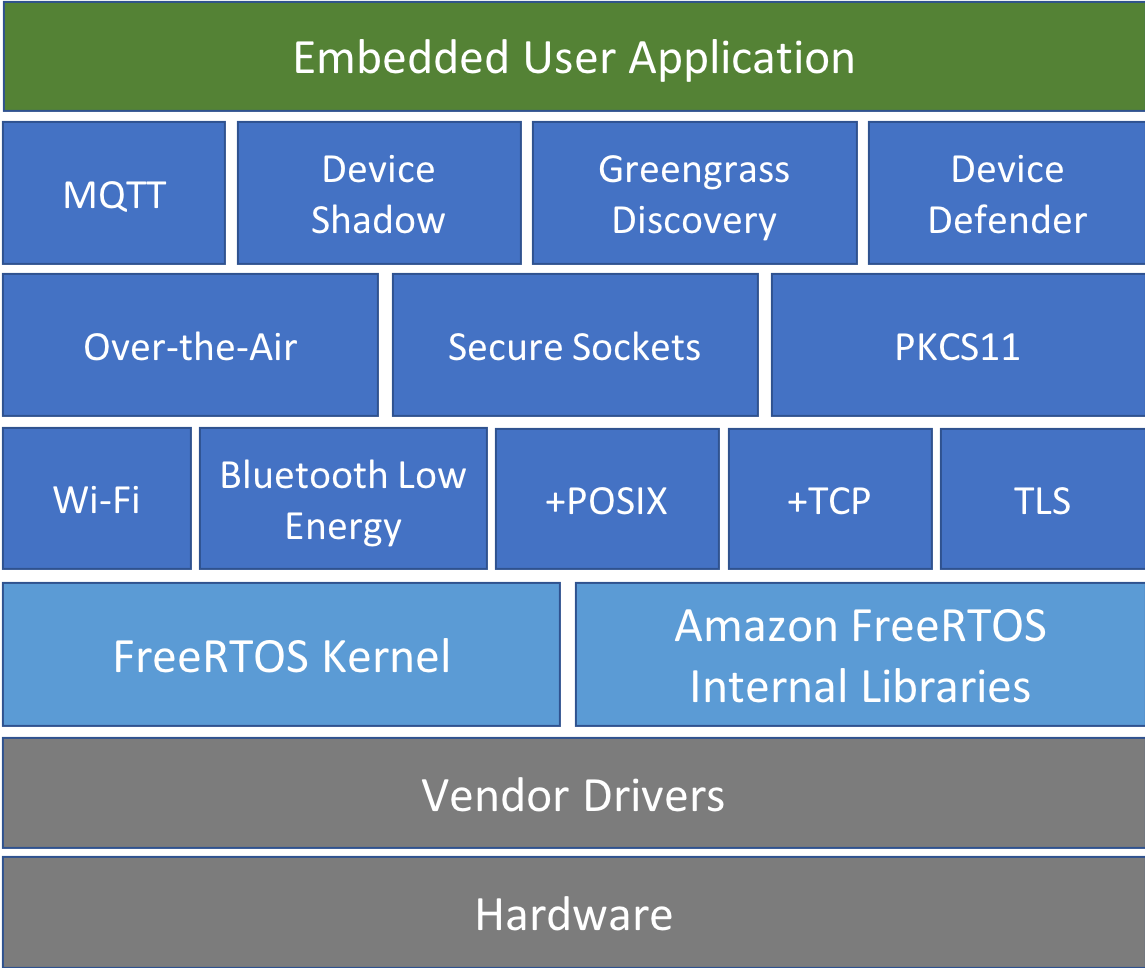
\includegraphics[width=0.75\textwidth]{figures/freertos-arch.png}
  \caption[FreeRTOS: arquitectura]{Arquitectura de FreeRTOS (kernel, librerías, drivers y hardware). Extraído de \parencite{freertos_official}.}
  \label{fig:arq-freertos}
\end{figure}


\subsection{Lenguaje de Implementación}
El sistema está escrito casi en su totalidad en C, con algunas porciones en ensamblador para 
la adaptación a diferentes arquitecturas de hardware, según se puede verificar en el repositorio 
oficial y la documentación de AWS \parencite{freertos_aws_docs}.

\subsection{Componentes Clave}
De acuerdo con su documentación oficial:
\begin{table}[H]
\centering
\begin{tabular}{p{3.2cm}p{5cm}p{6cm}}
\hline
\textbf{Componente} & \textbf{Función principal} & \textbf{Detalles clave / ejemplos} \\
\hline
Gestión de tareas & Coordinar la ejecución de múltiples hilos ligeros & Planificación basada en prioridades; soporte para multitarea con cambio de contexto rápido \\
\hline
Sincronización & Coordinar la comunicación entre tareas & Proporciona colas, semáforos, mutex y mecanismos de notificación \\
\hline
Memoria & Administrar la asignación dinámica de recursos & Ofrece cinco esquemas configurables (\texttt{heap\_1} a \texttt{heap\_5}) para distintas necesidades \parencite{freertos_getting_started} \\
\hline
Temporización & Gestionar eventos dependientes del tiempo & Incluye soporte para temporizadores de software, útiles en aplicaciones en tiempo real \\
\hline
Extensiones & Ampliar las capacidades del sistema & Librerías opcionales como FreeRTOS+TCP (red) y FreeRTOS+FAT (sistema de archivos) \\
\hline
\end{tabular}
\caption[Componentes y funciones clave de FreeRTOS]{Componentes y funciones principales de FreeRTOS. Basado en la documentación oficial \parencite{freertos_getting_started}.}
\label{tab:componentes-freertos}
\end{table}


\subsection{Comunidad y Documentación Disponible}
FreeRTOS cuenta con documentación exhaustiva en su sitio oficial, 
incluyendo manuales, ejemplos de uso y certificaciones de seguridad.  
La comunidad es muy amplia, con foros técnicos, repositorios públicos y soporte activo 
de AWS en la versión oficial de mantenimiento a largo plazo.

%------------------------------------
\section{macOS (Darwin/XNU)}

\subsection{Historia y Propósito}
Darwin es la base de macOS, iOS y otros sistemas de Apple. 
Su núcleo XNU combina Mach, BSD y el framework I/O Kit. 
\textcite{xnu_opensource} indican que Apple liberó gran parte de Darwin bajo licencia APSL en el año 2000, 
pero mantiene cerradas las capas superiores de macOS.  
El propósito de Darwin es servir como plataforma Unix moderna y flexible, 
aprovechando lo mejor de Mach (microkernel) y BSD (servicios POSIX) \parencite{xnu_github}.

\subsection{Arquitectura}
El kernel XNU es híbrido: integra Mach para la gestión de hilos y memoria, 
BSD para los procesos, la pila de red y los sistemas de archivos, 
y el framework I/O Kit en C++ para los controladores de hardware \parencite{darwin_documentation}.  
Esta arquitectura busca un equilibrio entre flexibilidad y rendimiento.

\begin{figure}[htbp]
  \centering
  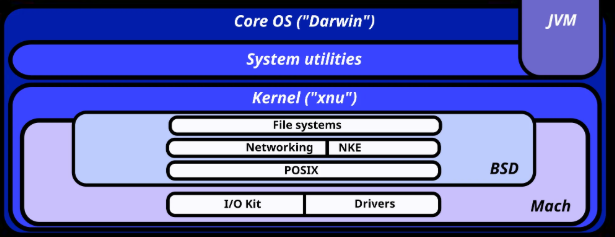
\includegraphics[width=0.65\textwidth]{figures/macos-arch.png}
  \caption[macOS (Darwin/XNU): arquitectura]{Arquitectura de macOS (Darwin/XNU). Extraído de \parencite{darwin_documentation}.}
  \label{fig:arq-macos}
\end{figure}

\subsection{Lenguaje de Implementación}
El kernel de Darwin está escrito principalmente en C (Mach y BSD) y C++ (I/O Kit). 
El resto del sistema (utilidades, librerías) se basa en C y componentes Unix heredados, 
como se documenta en los recursos oficiales \parencite{macos_architecture}.

\subsection{Componentes Clave}
De acuerdo con la documentación oficial:
\begin{table}[H]
\centering
\begin{tabular}{p{3.2cm}p{5cm}p{6cm}}
\hline
\textbf{Componente} & \textbf{Función principal} & \textbf{Detalles clave / ejemplos} \\
\hline
Mach & Gestionar memoria virtual, hilos e IPC & Proporciona multitarea, planificación de hilos, comunicación entre procesos y administración de memoria virtual \\
\hline
BSD & Ofrecer servicios POSIX y red & Maneja procesos POSIX, el sistema de archivos virtual y la pila de red TCP/IP \\
\hline
I/O Kit & Gestionar controladores de hardware & Marco orientado a objetos escrito en C++ que facilita la creación y carga dinámica de drivers \\
\hline
Darwin userland & Proporcionar entorno de usuario & Incluye el shell, utilidades básicas de Unix y bibliotecas estándar necesarias para aplicaciones \\
\hline
\end{tabular}
\caption[Componentes y funciones clave de macOS (Darwin/XNU)]{Componentes y funciones principales de macOS (Darwin/XNU). Basado en la documentación oficial \parencite{darwin_documentation}.}
\label{tab:componentes-macos}
\end{table}


\subsection{Comunidad y Documentación Disponible}
El código fuente de Darwin está publicado en Apple Open Source, 
incluyendo el kernel XNU, librerías y utilidades BSD.  
La comunidad activa está formada principalmente por desarrolladores del kernel, 
proyectos de investigación y entusiastas de sistemas Unix. Apple proporciona 
documentación detallada para desarrolladores del kernel.

\section{Haiku OS}

\subsection{Historia y Propósito}
Haiku es un sistema operativo iniciado en 2001 bajo el nombre OpenBeOS, 
renombrado en 2004, como una reimplementación libre de BeOS \parencite{haiku_official}.  
Su propósito es ofrecer un entorno de escritorio rápido, simple y coherente, 
centrado en la experiencia del usuario y la eficiencia del sistema \parencite{haiku_about}. 
\textcite{haiku_hackaday} destacan que el proyecto busca mantener viva la filosofía de BeOS en hardware moderno.

\subsection{Arquitectura}
El kernel de Haiku es híbrido, derivado de NewOS, con soporte de multiprocesamiento (SMP) 
y un sistema de archivos propio (BFS) con capacidades avanzadas de indexación y metadatos \parencite{haiku_github}.  
El sistema utiliza un modelo multihilo intensivo: cada ventana, aplicación y servicio 
funciona como un hilo separado.

\begin{figure}[H]
  \centering
  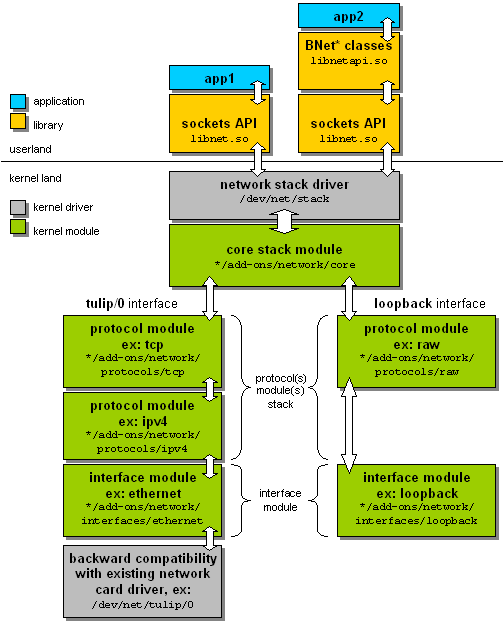
\includegraphics[width=0.75\textwidth]{figures/haiku_network.png}
  \caption[Arquitectura del \textit{Network Kit} de Haiku OS]{Arquitectura del \textit{Network Kit} de Haiku OS, basado en un stack modular con librerías compartidas, API POSIX/BSD y un stack driver que conecta el kernel con las aplicaciones. Extra\'ido de \parencite{haiku_network_kit}.}
  \label{fig:haiku_network}
\end{figure}

\subsection{Lenguaje de Implementación}
Haiku está escrito en C++98, con una API orientada a objetos para aplicaciones, 
drivers y componentes del sistema, como se puede verificar en su repositorio oficial.

\subsection{Componentes Clave}
Según la documentación oficial y análisis técnicos:
\begin{table}[H]
\centering
\begin{tabular}{p{3.2cm}p{5cm}p{6cm}}
\hline
\textbf{Componente} & \textbf{Función principal} & \textbf{Detalles clave / ejemplos} \\
\hline
Kernel NewOS & Administrar procesos y recursos del sistema & Soporta multitarea y multiprocesamiento; núcleo derivado de NewOS adaptado a Haiku \\
\hline
Sistema de archivos BFS & Gestionar almacenamiento con alto rendimiento & Soporta indexación, atributos extendidos y búsquedas rápidas en el sistema de archivos \\
\hline
Kits (APIs) & Proporcionar interfaces unificadas a desarrolladores & APIs para GUI, multimedia, red y almacenamiento, garantizando consistencia entre aplicaciones \\
\hline
App Server & Servir como gestor gráfico y de ventanas & Maneja la interfaz de usuario, el renderizado de ventanas y la comunicación con el hardware gráfico \\
\hline
Aplicaciones integradas & Brindar herramientas listas para el usuario & Incluye navegador WebPositive, gestor de archivos, cliente de correo y utilidades básicas del sistema \\
\hline
\end{tabular}
\caption[Componentes y funciones clave de Haiku OS]{Componentes y funciones principales de Haiku OS. Basado en la documentación oficial y análisis técnicos \parencite{haiku-docs}.}
\label{tab:componentes-haiku}
\end{table}


\subsection{Comunidad y Documentación Disponible}
Haiku es mantenido por voluntarios y coordinado por Haiku, Inc. 
El proyecto publica un manual de usuario, documentación de desarrollo y FAQs detalladas.  
La comunidad participa activamente en foros, listas de correo e IRC, 
con lanzamientos beta periódicos y nightly builds accesibles al público. 
El sistema ha ganado reconocimiento como un SO de escritorio funcional para uso diario.

\section{Android (AOSP)}

\subsection{Historia y Propósito}
Android fue desarrollado inicialmente por Android Inc. en 2003 y adquirido por Google en 2005. 
El \textit{Android Open Source Project} (AOSP) constituye la base abierta del sistema, 
distribuido para fabricantes y desarrolladores \parencite{aosp_source}.  
Su propósito es proveer una plataforma flexible, segura y abierta para dispositivos móviles 
y sistemas embebidos \parencite{android_developers}.

\subsection{Arquitectura}
\textcite{aosp_kernel} explican que Android se basa en un kernel Linux monolítico modificado por Google.  
Encima del kernel están la capa de abstracción de hardware (HAL), bibliotecas nativas 
(en C/C++ como Bionic libc), la Android Runtime (ART) para ejecutar aplicaciones en Java/Kotlin, 
y el framework de aplicaciones con servicios del sistema \parencite{aosp_architecture}.

\begin{figure}[H]
    \centering
    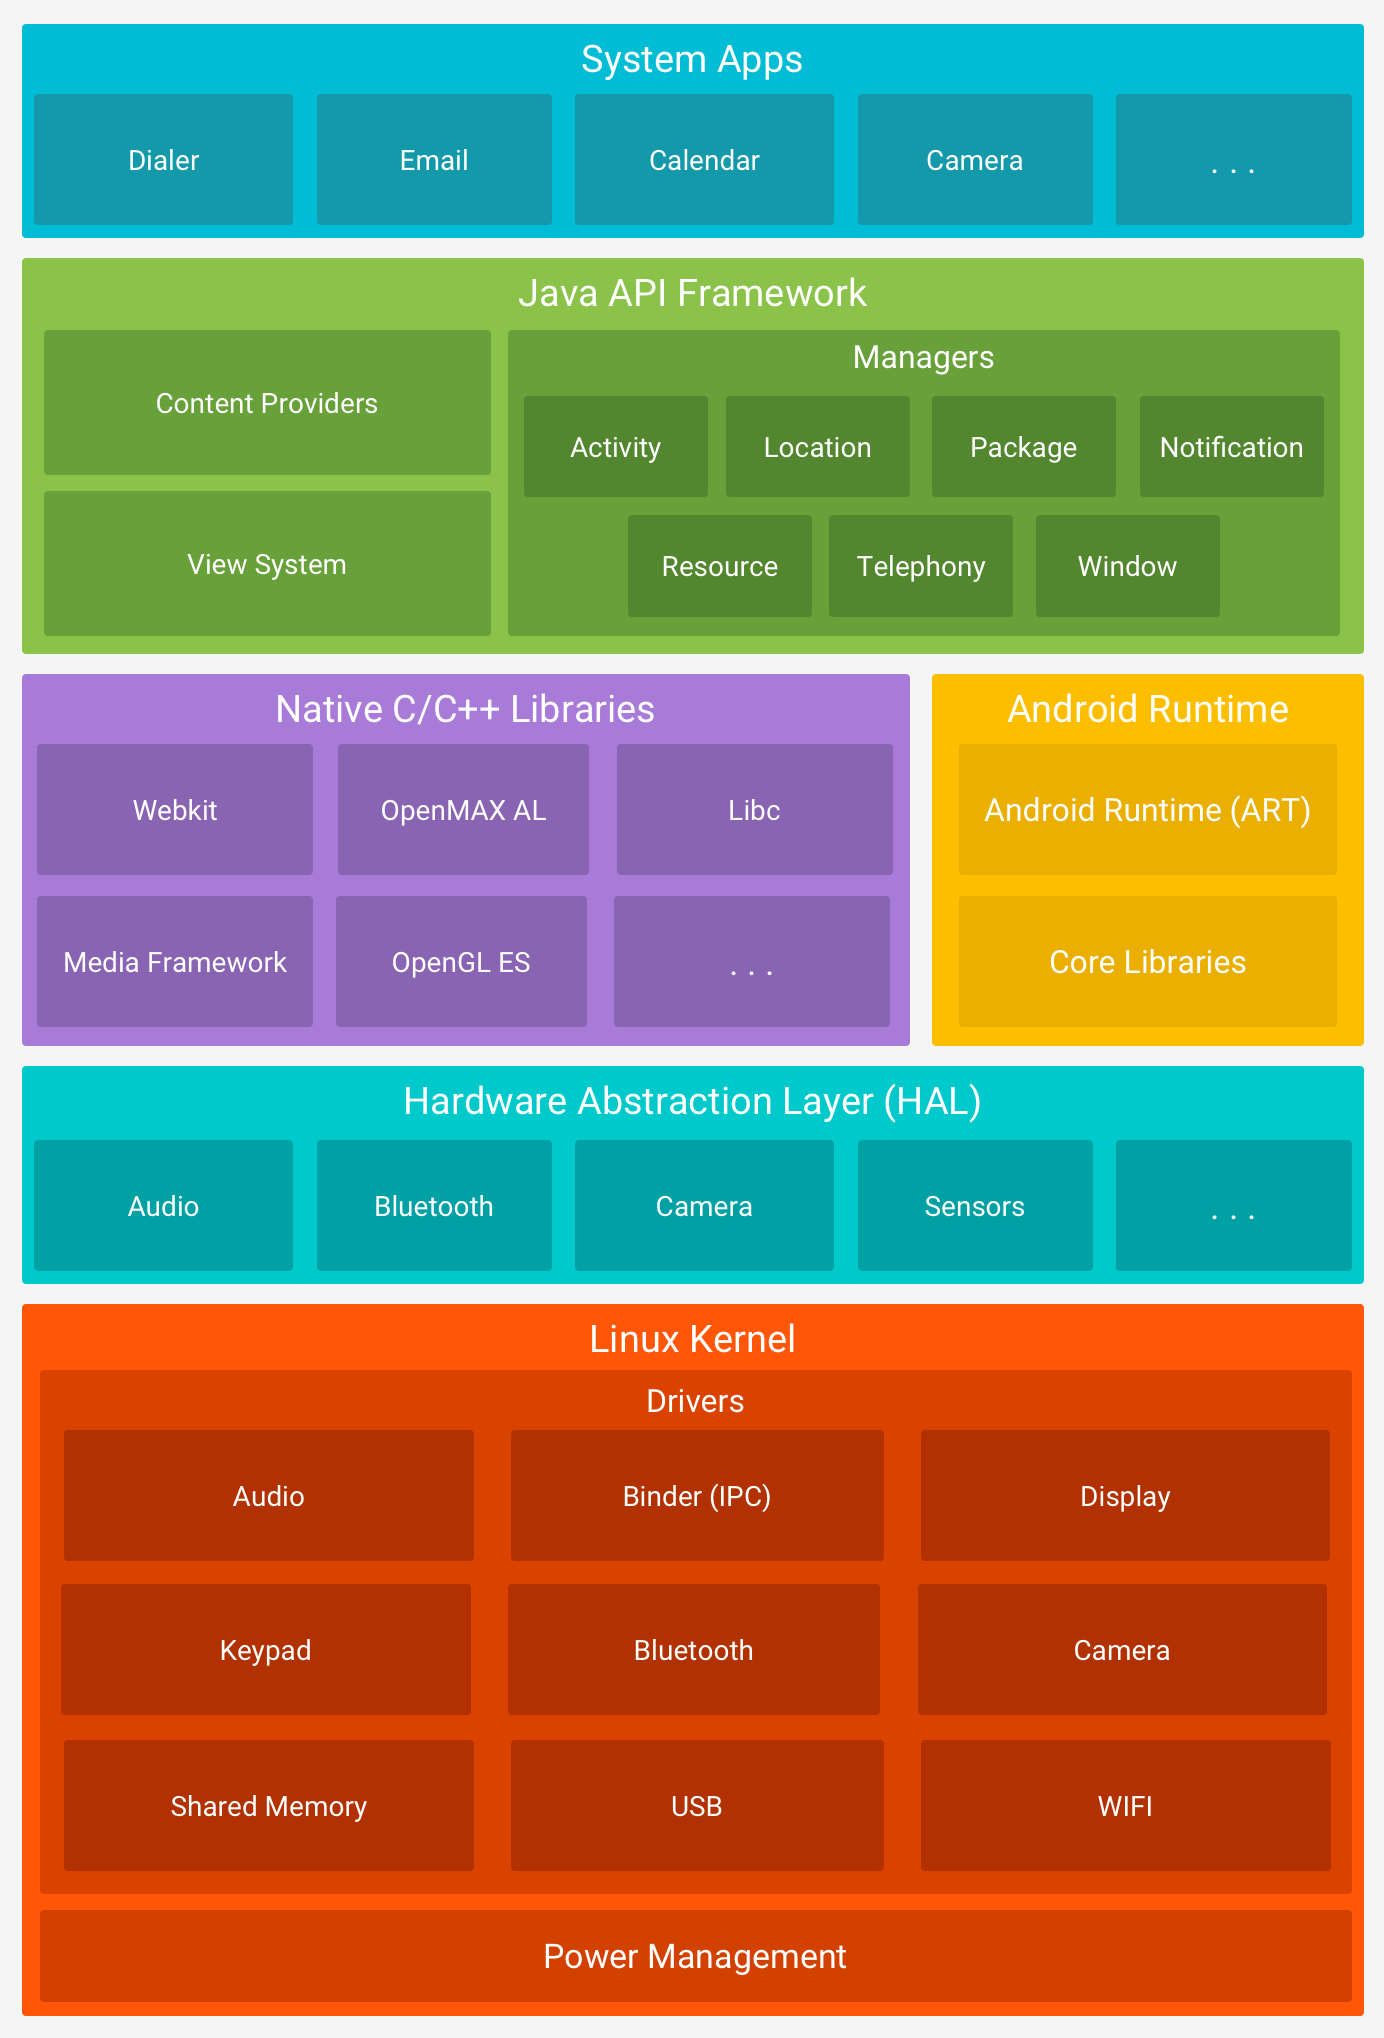
\includegraphics[width=0.75\textwidth]{figures/android_architecture.png}
    \caption[Arquitectura del sistema Android]{Arquitectura de la plataforma Android. Extra\'ido de \parencite{aosp_architecture}.}
    \label{fig:android_architecture}
\end{figure}

\subsection{Lenguaje de Implementación}
El kernel y las bibliotecas están escritos en C/C++, 
el runtime ART está en C++ y el framework superior en Java y Kotlin, 
según se documenta en las fuentes oficiales del proyecto.

\subsection{Componentes Clave}


\begin{table}[H]
\centering
\begin{tabular}{p{3.2cm}p{5cm}p{6cm}}
\hline
\textbf{Componente} & \textbf{Función principal} & \textbf{Detalles clave / ejemplos} \\
\hline
Kernel Linux & Administrar recursos básicos del sistema & Planificación de procesos, gestión de memoria, controladores de dispositivos \\
\hline
Binder & Proveer el mecanismo principal de comunicación entre procesos & IPC nativo de Android; utilizado por aplicaciones y servicios del sistema \parencite{aosp-docs} \\
\hline
ART (Android Runtime) & Ejecutar aplicaciones Android de forma eficiente & Soporta compilación JIT (Just-In-Time) y AOT (Ahead-Of-Time) para mejorar rendimiento \\
\hline
Framework & Ofrecer servicios de alto nivel a las aplicaciones & Incluye \textit{System Server}, \textit{SurfaceFlinger}, servicios de ubicación, telefonía, entre otros \\
\hline
Almacenamiento & Gestionar persistencia de datos y archivos & Usa sistemas de archivos EXT4 o F2FS; motor de base de datos integrado SQLite \\
\hline
\end{tabular}
\caption[Componentes y funciones clave de Android]{Componentes y funciones principales de Android (kernel 3.10.4). Basado en la documentación de AOSP \parencite{aosp-docs}.}
\label{tab:componentes-android}
\end{table}


\subsection{Comunidad y Documentación Disponible}
La documentación oficial está en el portal de AOSP, 
que incluye guías de arquitectura, compatibilidad (CDD) y código fuente completo.  
Google mantiene repositorios y foros para fabricantes y desarrolladores, 
mientras que la comunidad global contribuye en ROMs, kernels y proyectos derivados.